\documentclass[a4paper, 12pt]{report}

\usepackage[utf8]{inputenc} %pour avoir les accents
\usepackage[T1]{fontenc} %pour gerer où couper les mots et les accents dans le pdf
\usepackage[francais]{babel} % pour avoir la typo francaise
\usepackage[a4paper]{geometry} % s'adapte à une feuille a4
\usepackage{setspace} % gere les espaces entre les lignes
\usepackage{color} %gere les couleurs
\usepackage{listings} % pour avoir des lignes de codes
\usepackage{hyperref} % gere les url
\usepackage{amssymb}  %pour les formules de math
\usepackage{graphicx} % pour gerer les images
%\usepackage[nottoc]{tocbibind} % gere la bibliographie

\begin{document}

%%%%%%%%%%%%%%%%%%%%%%%%%%%%% Page de garde
\begin{titlepage}

%%%%%% Entête
\begin{figure}[t]
\begin{center}

\includegraphics[width=0.45\textwidth]{ub.png}

\includegraphics[width=0.45\textwidth]{scrime.png}
\end{center}
\vspace{1cm}
\end{figure}

\begin{center}
{\LARGE Licence d'Informatique\\Rapport de Stage\\Du 5 novembre 2015 au 27 juin 2016\\}
\end{center}
%%%%%% Fin Entête

%%%%%% Titre
\begin{center}
\vspace{1.4cm}
\fbox{
	\begin{minipage}{\textwidth}
	\begin{center}
	{\color{cyan} \Huge Interface de pilotage \\du robot "Thymio" avec I-score\\}
	\end{center}
	\end{minipage}
	}
\end{center}
%%%%%% Fin Titre	
\vspace{1.4cm}

%%%%%% Personnes
\begin{description}
\item[{\LARGE Stagiaire:}{ Gaëtan CHAMBRES}]
\item[{\LARGE Responsable de stage:}{ Pierre COCHARD}]
\vspace{0.5cm}
\item[{\LARGE Co-dirigeant de stage:}{ Phillipe GUILLEM}]
\end{description}

%%%%%% Fin Personnes
\vspace{1.4cm}
%%%%%% Adresse
\begin{description}
\item[Stage effectué au sein de:]
\item[Université de Bordeaux]
\item[351 cours de la libération]
\item[33405 Talence cedex]
\end{description}

%%%%%% Fin Adresse


\end{titlepage}
%%%%%% fin de la page de garde


\chapter*{Remerciements}
\pagenumbering{roman}

Tout d'abord, d'adresse toute ma gratitude à Monsieur Pierre COCHARD, en qualité de maître de stage, ainsi qu'a Monsieur Philippe Guillem, pour leur disponibilité, leur soutien, leur compréhension et leur attention. Leur confiance et le partage de leurs connaissances ont fait de ce stage un apport crucial de connaissances et d'expériences.\\

Je tiens également à remercier Madame Annnick Mersier pour son aide et son soutien tout au long de l'année, ainsi que pour son acceuil chaleureux à elle et à toute l'équipe du SCRIME.\\
Je souhaite aussi remercier Madame Myriam Desainte-Catherine pour sa confiance et sa compréhension lors de ma première démarche, grâce à qui ce stage à pu voir le jour.\\\\
J'adresse également mes remerciements à toutes les personnes qui ont pu m'aider lors de mes recherches durant ce stage, toutes celles qui auront lu et répondu à mes mails de questionnement, et en particulier à Mr Didier ROY qui aura été un contact précieux à l'INRIA, notemment pour le prêt d'un robot Thymio afin d'effectuer mes premiers tests.\\\\
Je souhaite aussi remercier Madame Émilie DOS SANTOS pour sa disponibilité, son dynamisme et sa réactivité qui ont permis d'organiser au mieux ce stage.\\

Pour finir, je tiens à remercier mon entourage et mes proches qui m'ont soutenu toute l'année, tant dans mes études que dans ce stage, ainsi que ceux qui m'ont conseillé dans la rédaction de ce rapport, ou bien qui l'ont relu.

\chapter*{Résumé}
	Ce stage, effectué au Studio de Création et de Recherche en Informztique et Musique Électroacoustiques (SCRIME), lié à l'équipe Image et Son du Laboratoire Bordelais de Recherche en Informatique (LaBRI) s'intéresse au robot pédagogique Thymio, et en particulier aux moyens de le rendre capable de jouer de la musique.\\
Une première partie est consacrée la présentation du robot Thymio et du projet qui lui a donné vie. Une seconde partie présente les possibilité natives de Thymio concernant le son, tandis qu'une troisième partie détaillera comment ce stage à permis d'étendre ces possibilités.\\
Pour finir, ce rapport présente l'archive du travail rendu ainsi que les possibilités d'amélioraitons et les suites prévues pour ce projet.

\tableofcontents %génére la table des matieres

\chapter{Introduction}
\pagenumbering{arabic} % reinitialise le compteur et numerote les pages en chiffres arabes
\section{Domaine du Stage}
\subsection{Le SCRIM}
Ce stage a été effectué au sein du Studio de Création et de Recherche en Informatique et Musiques Expérimentales( ou Électro-acoustiques).\\
Ce groupement d'intérêt scientifique et artistique est rattaché à l'équipe Image et Son du Laboratoire Bordelais de Recherche en Informatique (LaBRI).\\
Les champs d'activités du SCRIME s'étendent de la recherche scientifique à la création artistique, en passant par la formation, la diffusion des musiques contemporaines et la pédagogie en milieu scolaire et universitaire. \\
Le SCRIME est soutenu par le Ministère de la Culture, le Conseil Régional d'Aquitaine, la DRAC et le CNRS.\\

\subsection{Les missions du SCRIME}
Les différentes missions du SCRIME sont:
\begin{itemize}
\item Favoriser la collaboration entre scientifiques et artistes à des fins de recherche et de création
\item Favoriser la diffusion internationale des résultats des recherches et des oeuvres artistiques
\item Promouvoir les collaborations scientifiques et artistiques avec d'autres centres de recherche et de création en France ou à l'étranger
\item Favoriser les actions pédagogiques dans les institutions partenaires ainsi que dans les autres établissements publics d'enseignement et de création et ce à tous les niveaux 
\end{itemize}

\subsection{L'équipe du SCRIME}
L'équipe de ce groupement d'intérêt scientifique et artistique est essentiellement composée de:
\begin{description}
\item[Myriam Desainte-Catherine :] Direction scientifique
\item[Jean-Louis Agobet :] Direction artistique
\item[Gyorgy Kurtag :] Coordination Arts et Sciences
\item[Annick Mersier :] Gestionnaire
\item[Christian Faurens :] Assistant ingénieur audiovisuel
\item[Pierre Cochard :] Réalisateur en Informatique Musicale
\item[Antoine Hubineau :] Chargé de communication
\item[Julia Hanadi Al Abed :] Régisseur son
\item[Jean-Michel Rivet :] Compositeur et Enseignant
\item[Raphaël Marczak :] Ingénieur de recherche
\item[Nicolas Vuaille :] Développeur
\end{description}
Pierre COCHARD  aura été mon responsable de stage, mais j'ai également travaillé avec Philippe GUILLEM, professeur de musique et enseignant en classe de maternelle.

\section{Le contexte du stage}
\subsection{Pourquoi ce projet?}

Philippe GUILLEM est maître formateur en musique et enseignant en école maternelle. Son objectif est de montrer à ses élèves ce que le monde moderne leur offre. Cela va des réseaux sociaux à la robotique, en passant par la programmation de manière plus vaste. Seulement une interrogation naissait en même temps que cette idée :\\

Comment chez des élèves de 5 ans, aider à construire une image du Robot et des relations que l'homme peut entretenir avec ces machines?\\

Lors d'une conférence, Philippe GUILLEM a découvert le projet du robot THYMIO. De part sa robustesse, sa simplicité d'accès, d'utilisation et de programmation, ainsi que par sa conception, il était tout à fait adapté aux jeunes enfants et donc à ce projet.
Enfin, il restait la question de représenter la relation homme / robot. Pour cela, Mr GUILLEM a tenu à faire un lien avec la musique, car c'est ce qu'il y a de plus parlant pour les jeunes auditorats. C'est donc à ce moment que le SCRIME a été sollicité, en particulier Pierre COCHARD, et ils ont travaillé sur le projet de ce stage.


\subsection{Les objectifs du stage}
L'objectif initial de ce stage était de réaliser une interface permettant de piloter le robot Thymio avec le logiciel I-score afin d'en permettre l'utilisation en classe avec des élèves de maternelle par monsieur Phillipe GUILLEM. \\
Dans ce but, ce stage devait permettre l'implémentation d'un système de communication entre Pyo (ou tout autre logiciel adapté) et le logiciel I-score.\\
Or le stage étant très étalé, mais d'une durée effective courte, les objectifs ont été redéfinis. L'objectif du stage est devenu d'écrire un programme permettant de traiter les évènements de Thymio extérieurement au robot, mais en temps réel. En effet, si ce traitement est valide, il devient aisé d'y insérer une transmission en protocole Open Sound Control (OSC) par exemple et ainsi de communiquer avec I-score.
L'objectif pédagogique était d'obtenir des compétences en robotique et dans le traitement des informations d'un capteur. 

\section{Contenu du rapport}
Afin de mieux comprendre la finalité de ce stage, ce rapport va d'abord permettre de définir ce qu'est Thymio et le projet pédagogique et communautaire auquel il appartient. 
Les fonctionnalités du robot seront ensuite détaillées, principalement ses compétences relatives au son et à la musique. Ensuite, seront expliqués les méthodes envisagées et sélectionnées afin d'étendre les compétences de base de Thymio. 
La partie suivante concernera l'archive finale de travail, ainsi que son contenu.
Enfin, une conclusion détaillera les résultats obtenus, les apports réalisés et les améliorations possibles.

\chapter{Le Robot Thymio}
\section{Présentation}

Thymio, conçu par l’École polytechnique fédérale de Lausanne, est un petit robot dédié à la pédagogie. Ses deux roues lui permettent déplacements et manoeuvres, tandis qu'il embarque des boutons ainsi que de nombreux capteurs infrarouges pour détécter des obstacle ou des surfaces, un micro, un haut parleur, un accéléromètre et même un thermomètre. Son accessibilité est due à la mise à disposition de ses propres interfaces de programmation. Il y en a en effet plusieurs, à commencer par l'interface de programmation texte, ASEBA STUDIO qui permet d'exploiter entièrement le langage ASEBA. Une adaptation de BLOCKY est aussi disponible, qui permet d'aborder la programmation texte de manière simplifiée, et enfin il y a VPL qui permet de programmer THYMIO visuellement grâce à des vignettes. C'est grâce à ces interfaces que ce robot se trouve adpaté aux plus jeunes.

Pour résumer, il s'agit d'un robot complet, qui embarque un grand nombre de capteurs, et accessible à tous, aux plus jeunes comme aux programmeurs confirmés, c'est pourquoi ce robot a été choisi pour ce projet de stage.

\section{Philosophie d'un projet collaboratif}
Le but du projet THYMIO était de permettre à un large publique, et en particulier aux enfants, la découverte et l'apprentissage de la programmation, de la robotique, de l'ingénierie et des technologies numériques. Pour permettre cela, il a fallut regrouper plusieurs corps de métiers et des connaissances poussées dans différents domaines. C'est pourquoi THYMIO est un projet communautaire, qui implique plusieurs entités. Il s'agit donc d'un modèle basé sur le partage libre des connaissances, c'est à dire que Tout le matériel, le logiciel, et la documentation sont développés par les partenaires sous licence libre. Ainsi, les partenaires s'engagent à fournir l'information de conception gratuitement, de manière à ce que chacun puisse comprendre, utiliser, ou modifier cette information, à condition de distribuer à son tour les résultats de son travail. Il est donc important que ce stage s'inscrive dans cette dynamique, et que le travails ainsi que les résultats soient partagés à la communauté.

\section{Les différents acteurs du projet}
Comme expliqué précédemment, plusieurs catégories d'acteurs se sont alliés dans ce projet:
\begin{description}
\item[Les institutions de recherche: ]qui permettent de diffuser le travail et de l'amener auprès du public. Plus la base d'utilisateurs grandit, meilleures sont les possibilités d'évaluation et d'amélioration. Les résultats de la recherche sont ainsi mis rapidement en application.
\item[Les entités de production: ] qui donnent accès à des produits proches de l'état de l'art qui n'ont plus qu'à être industrialisés. Les frais liés à des licences sont réduits et les produits sont validés scientifiquement. Les entités de production distribuent toute l'information (schémas, plans, pdf des exercices, etc.) gratuitement et commercialisent les supports physiques (robots, accessoires, livrets imprimés, etc.).
\item[Les contributeurs] permettent de participer à un grand projet selon ses moyens et de choisir son implication, de proposer des idées, de recevoir de l'aide et de l'information et de voir son travail diffusé.
\item[Les utilisateurs] leur apport se perçoit dans du matériel moins cher, beaucoup de ressources gratuites, une transparence dans le projet, et une plus grande pérennité du produit.
\end{description}

Parmis les principaux acteurs, on pourra citer en particulier:
\begin{description}
\item[EPFL - École Polytechnique Fédérale de Lausanne] Initiatrice du projet.
\item[Association Mobsya] Association responsable de la production et de la distribution du robot.
\item[ETH - Eidgenössiche Technische Hochschule Zürich] Le laboratoire de Systèmes Autonomes et le centre de technologies de jeu de l'ETH Zürich qui ont contribué à ASEBA et à VPL.
\item[NCCR Robotics] Aide financière et aide à la validation scientifique.
\item[la Loterie Romande, Suisse]
\item[et le Fond National Suisse de la Recherche Scientifique] Respectivement pour l'aide financière pour les premières production et l'aide financière pour la mise en place de kits éducatifs
\item[INRIA - L'Institut National de Recherche en Informatique et en Automatique] Développeur principal de l'adaptation de SCRATCH au THYMIO, qui donnera BLOCKY, et développement du matériel éducatif pour les enseignants, notamment avec le projet "Dessine-moi un robot". 
\end{description} 

L'INRIA nous aura grandement aidé dans notre projet, grâce notamment au contact de Didier Roy; docteur en informatique cognitive, lié de près au projet Thymio, qui nous aura aidé dans nos réfléxions, mais aussi prêté un THYMIO de test pendant plusieurs mois avant que le SCRIME n'ai pu en faire l'acquisition.

\section{Les engagements de la société créatrice}
Pour suivre cette philosophie basée sur la collaboration et les sources ouvertes (open source), la société créatrice a choisi les modes de diffusion suivants:
\begin{itemize}
\item pour le logiciel, le code source est en open source, sous licence LGPL.
\item pour le matériel, sont distribués tous les documents de conception, y compris schémas électronique, plans des pièces, etc. en open hardware sous une licence CC-BY-SA 3.0
\item pour la documentation, les exercices, les cursus, sont distribués également tous les documents en format numérique sous une licence CC-BY-SA 3.0.
\end{itemize}

Afin de permettre une production et un distribution à grande échelle, une association à but non lucratif a été crée, Mobsya. L'association assure la production du matériel. Pour le logiciel, elle contribue à la maintenance et au développement en collaboration avec les autres partenaires. L'association gère aussi l'infrastructure qui permet de créer une communauté d'utilisateurs, qui peuvent s'entraider grâce à des listes de discussion et un site de partage d'information qui contient la documentation, des exemples de réalisation, du support technique, etc. Cette infrastructure aura également aidé durant ce stage.

\chapter{Les fonctionnalités de Thymio concernant le son}
\section{Les fonctionnalités natives de Thymio}
Le robot Thymio est déjà conçu pour une intéraction basée sur le son. C'est possible entre autre grâce à la présence d'un micro et d'un haut-parleur, mais aussi grâce au slot micro-SD. Seulement les possibilité sont limitées.

\subsection{Intensité sonore ambiante}
Le robot peut détecter lorsque le bruit ambiant est au-dessus d'une intensité donnée. C'est possible, grâce à la variable mic.intensity qui donne l'intensité du microphone embarqué ou encore grâce à la variable mic.threshold qui contient la limite de l'intensité pour l'événement. Un évènement est alors généré si mic.intensity est au-dessus de mic.threshold.\\

\section{La synthèse sonore de Thymio}
\subsection{la Génération de sons}
Le langage Aseba possède une fonction native "sound.freq" qui joue une fréquence, spécifiée en Hz, pour une certaine durée, spécifié dans 1/60 s. Une durée égale à 0 joue le son à l'infini et une durée de -1 arrête le son.\\
La génération de sons de synthèse fonctionne par ré-échantillonnage d'une onde primaire. Par défaut, l'onde est triangulaire, mais il est possible de la	définir à l'aide de la fonction native "sound.wave". Cette fonction prend en entrée un tableau de 142 échantillons, avec des valeurs de -128 à 127. Ce tableau doit représenter une onde tonique de la fréquence spécifiée dans sound.freq.\\
 Comme Thymio joue des sons à 7812,5 Hz, ce tableau est joué entièrement à la fréquence de 7812.5/142 = ~ 55 Hz. Jouer un son de fréquences plus élevées fait sauter des échantillons dans le tableau.

\subsection{L'enregistrement et la relecture}
Il est aussi possible d'enregistrer des sons en utilisant la fonction native "sound.record" qui prend en paramètre un numéro d'enregistrement de 0 à 32767. Le fichier est stocké sur la carte micro-SD sous le nom Rx.wav où x est le paramètre passé à la fonction sound.record. Pour arrêter un enregistrement, il faut appeler la fonction sound.record avec la valeur -1.\\
On peut également rejouer un son enregistré en utilisant la fonction native sound.replay . Cette fonction prend en paramètre un nombre de 0 à 32767 et rejouer le fichier Rx.wav de la carte SD où x est le paramètre passé à la fonction sound.replay. Pour arrêter une lecture, il faut appeler la fonction sound.replay avec une valeur de -1.

\subsection{La lecture de "Sample"}
Il est également possible de jouer d'autres sons que les sons simples générés par synthèse ou les sons système. En utilisant une carte micro-SD formatée FAT, il est possible d'enregistrer et de jouer des "samples", des morceaux de musique pré-enregistrés. Les fichiers doivent cependant être stockés sur la carte micro-SD au format wave, 8-bit non-signé, 8 kHz. Lorsque le robot fini la lecture d'un son demandée par ASEBA, il déclenche l'événement sound.finished . Il ne se déclenche pas d'événement si la lecture est interrompue ou si un nouveau son est joué.\\

\subsection{La création de son depuis un ordinateur}
Voici la démarche, selon les créateurs de Thymio, pour créer, à l'aide du logiciel Audacity, un son compatible avec Thymio II qui puisse être joué:\\
\begin{itemize}
\item Une fois démarré audacity, changer le "project rate" situé en bas à gauche de 44100 Hz (défaut) à 8000 Hz.
\item Enregistrer le son avec la touche record rouge en haut à gauche. Le curseur doit avancer et la forme d'onde se visualiser. Stopper une fois fini avec le bouton stop.
\item Le son doit être en mono (Piste->Piste stéréo vers mono)
\item Aller sur le menu File sous Export…
\item Donner un nom de ficher.
\item Choisir comme format: other uncompressed files.
\item Sous "options" choisir un header WAV (Microsoft) et comme "Encoding" choisir Unsigned 8 bit PCM.
\item Sauver ou copier le ficher sur une carte micro-SD.
\end{itemize}

\subsection{Sons système}
Les sons système de Thymio peuvent être utilisés à l'aide de la fonction native "sound.system" , qui prend un nombre de 0 à 32767 en tant que paramètre. Certains sons sont disponibles dans le firmware (voir ci-dessous), mais on peut remplacer ces sons et en ajouter de nouveaux en utilisant la carte micro-SD. Pour arrêter la lecture d'un son, il faut rappeler la fonction sound.system avec la valeur -1.

\subsection{Bibliothèque de son système}
Les sons suivant sont disponibles :\\
paramètre 	description\\
-1 	arrête de jouer un son\\
0 	son de démarrage\\
1 	son d'arrêt (son non reconfiguration)\\
2 	son des boutons fléchés\\
3 	son du bouton central\\
4 	son de chute libre (peureux)\\
5 	son de choc\\
6 	son de suivi d'objet\\
7 	son de détection d'objet pour suivi\\
Pour ne plus entendre de son système, vous pouvez décompresser sur une carte micro-SD cette archive qui contient des sons muets.

\section{Les limites}
Cette gestion du son de par les fonctions natives de Thymio est assez limitée. En effet, il est seulement possible de lire des sons soit du système, soit des sons pré-enregistrés. Ces sons doivent être échantillonés a 8kHz, ce qui impacte fortement leur qualité. Quant à la synthèse, il faut se contenter de jouer des fréquences en utilisant des ondes primaires, comme indiqué précemment. C'est pour ces raisons que l'objectif de ce stage sera d'établir un protocole de communication entre Thymio et l'ordinateur de manière à ce que ce soit le PC qui synthétise le son en fonction des informations communiquées par le robot.

\chapter{L'extension des possibilités sonores de Thymio}
\section{Les outils informatiques utilisés}
La réalisation de ce stage aura nécessité la combinaison de plusieurs outils, tels que le langage Aseba, le langage C, l'hébergement de projet sur git, la programmation système ou encore la recherche sur forums et canaux de discussion.

\subsection{Le langage de programmation Aseba}
Le langage Aseba est un langage spécialement adapté pour la programmation de comportements pour robots à micro-contrôleurs. Ce langage open source est une architecture de contrôle temps réel et distribué de robot mobile, basée sur la programmation évènementielle. Aseba dispose de son propre environnement de développement (Aseba Studio) qui est totalement intégré au robot Thymio. C'est pour cela que ce langage a été utilisé lors de ce stage. Sémantiquement, il s'agit d'un langage de programmation impératif avec un seul type simple (nombres entiers signés sur 16 bits) et des tableaux.

\subsection{Les outils ASEBA}
Mais Aseba c'est aussi un ensemble de programme et d'outils qui peuvent permettre d'aider la programmation de robots. En témoigne l'installation des programmes tels que "asebadump", "asebaswitch", "asebaexec", "asebaeventlogger", etc...
Certain seront étudiés, comme asebaexec ou asebadump, d'autre serviront directement lors de la réalisation du travail comme asebaswitch.

\section{L'externalisation des événements}
Le stage s'étalant sur une durée effective relativement courte (4 semaines de travail), il aura été principalement articulé autour de la possibilité d'externaliser les évènements générés par le robot lors de la stimulation de ses capteurs. Il est nécessaire de pouvoir traiter les données des cpateurs depuis l'ordinateur récepteur, et de cette manière, une synthèse sonore précise et de haute qualité peut être calculée.

\chapter{La réalisation de cette extension}
\section{La communication entre Thymio et un ordinateur}
Au cours de ce stage, deux générations de Thymio auront été étudiées, le Thymio II et le Thymio II Wireless. La seule différence se fait d'un poinit de vue matériel, puisque que le Thymio II Wireless permet de s'affranchir du câble USB qui le relie à l'ordinateur. Tout l'intérêt de cet investissement réside dans le fait de pouvoir maintenir la communication antre l'ordinateur et le robot peu importe la distance, sa place dans le parcours et la taille de celui-ci. En revanche, d'un point de vue logiciel, il n'y à pas de différence, l'ordinateur capte les valeurs des capteurs de la même manière, que ce soit par USB ou par radiofréquence.

\section{L'idée principale}
Premièrement, il a fallu mettre en place un code Aseba qui génère des évènements lorsque cela est souhaité, autrement dit à chaque stimulation de capteurs. Grâce à l'étude de la documentation de Aseba, l'idée d'utiliser la fonction "emit" est apparue assez naturellement. Elle est définie ainsi:

\begin{itemize}
\item{\textit{Un script peut envoyer des événements en utilisant le mot clé emit, suivi par le nom de l'événement ainsi que du nom de la variable à envoyer. [...] Les événements permettent ainsi à un script de déclencher l'exécution de code sur un autre nœud ou de communiquer avec un programme externe.}}
\end{itemize}

Suite à l'écriture de se programme, le robot envoie bien des évènements. Ceux-la sont visible dans la fenêtre dédiée d'Aseba Studio. Il était alors possible de lancer une partie du code à executer sur le Thymio en fonction de l'évènement envoyé, mais le problème n'était pas résolu, cela ne suffisait pas à externaliser complètement les évènements.

Après étude du code source d'Aseba et de celui des outils qui lui sont relatifs, le manque de solutions aura nécessité des recherches au sein de la "communauté Thymio". C'est en cherchant de l'aide sur le forum principal d'Aseba que l'idée d'inscrire les évènements dans un fichier texte est apparue.\\
En effet, il est possible de faire en sorte que chaque évènement envoyé ainsi que les données qui s'y rapportent soient inscrites dans un fichier texte en temps réel. Une fois cette méthode lancée, la lecture de se fichier permet d'analyser les données des évènements et de les traiter comme on le souhaite, ce qui est l'objectif principal de ce stage.

\section{L'écriture dans un fichier texte}
Il existe donc des commandes qui permettent l'écriture dans un fichier texte de la totalité des évènements envoyés. Pour cela, il faut se connecter au port sur lequel est connecté le robot Thymio afin de lire les données envoyées grâce à la commande :
\begin{verbatim}
~/asebaswitch "ser:name=Thymio"\\
\end{verbatim}
 
Il faut ensuite indiquer par une commande que l'on souhaite enregistrer la totalité des données passantes par ce port dans un fichier avec la ligne:
\begin{verbatim}
~/asebarec "tcp:localhost;port=33333" > <nom_du_fichier>
\end{verbatim}
 

A la suite de ça, on peut executer, sur le robot, le code écrit dans aseba et voir s'inscrire en temps réel les données des évènements dans le fichier passé plus tôt en paramètre.

\section{La lecture du fichier texte}
Une fois le résultat souhaité obtenu en écriture, il reste à lire le fichier. Pour cela, il y a le programme "loop\_read". Ce programme prend deux paramètres, le nom du fichier dans lequel les évènements sont ecrits, et le nom d'un second fichier, au choix de l'utilisateur dans lequel chaque donnée des évènements traités sont écrites proprement avec leur signification. Cela permet d'avoir une trace de fonctionnement du programme, des évènements traités et donc de leur nombre.\\
La principale difficulté aura été de faire en sorte que le programme de lecture fonctionne en même temps que l'écriture, et que tous les évènements soient traités en temps réel. Pour cela, le programme "loop\_read" scanne le fichier des évènements ligne par ligne (on sait qu'a une ligne correspond un évènement). Si le numéro d'identifiant de l'évènement est différent de celui traité précédemment, alors on le traite. Sinon, on scanne la ligne suivante. Cet algorithme permet de s'assurer que la totalité des évènements déjà ecrits sont traités, et qu'il n'y ai pas de répétition d'évènements. La dernière modification consiste à répéter cet algorithme tant que l'évènement final n'est pas détécté. L'évènement final est celui identifié par la constante NBR\_STOP\_EVENT en début du fichier. Il s'agit d'un évènement à part qui va déterminer que l'on termine le programme à son émission.


\chapter{Le contenu de l'archive finale}
\section{Le README}
L'archive finale contient différents fichiers qui sont nécessaires pour l'éxécution de ce code. Elle contient en particulier un fichier "README.md" qui détaille le contenu des autres fichiers de l'archive mais aussi qui sert de guide pas-à-pas au lancement du programme de traitement des évènements.

\section{Makefile}
Le makefile présent est aussi simple qu'il est efficace. Il permet de compiler le programme "loop\_read".

\section{Le fichier Aseba}
Ce fichier ("prox-event-sender.aesl") contient le code d'exemple qui sera à exécuter sur le robot. Il ne prend pas en charge de déplacements, seulement la gestion des évènement en fonction de la stimulation des capteurs de proximité horizontale. Il est extensible à n'importe quel autre capteur, et intégrable à d'autre codes Aseba.

\section{Le fichier loop\_read}
Il s'agit du programme principal. Il est nécessaire d'ajuster la constante \\NBR\_STOP\_EVENT en fonction de l'identifiant donné à l'évènement final qui est déterminé dans le code du fichier Aseba. Les autres modifications à apporter concerneront le traitement plus fin des données des évènements (la transmission en protocole de communication avec un séquenceur par exemple). Ce traitement sera à insérer dans ce programme à l'endroit indiqué par les commentaires ou par le README.

\chapter{Bilan}
\section{Apports du stage sur le plan personnel}
Ce stage aura été très particulier. En effet, il se sera étalé tout au long de l'année scolaire de début Novembre à début fin Mai, tandis que le temps de travail effectif aura été très court, puisque cela correspond à environ 4 semaines. Cette organisation très particulière aura été difficile à gérer. En effet, il aura été compliqué de concilier convenablement les cours, les projets et les examens en plus du stage. Cependant, cela m'aura appris à m'organiser à long terme, car c'est ainsi que ce stage a pu aboutir. Une autre leçon principale aura été de me rendre compte a quel point il était important d'avancer efficacement car en me présentant seulement une demi-journée par semaine, il fallait optimiser mon avancée sur cette demi-journée.\\
Ensuite, le fait de travailler sur le robot Thymio, et au coeur du projet pédagogique qui l'entour, m'aura appris à travailler sur un projet libre. C'est à dire que cela m'a appris a contacter des personnes afin de demander de l'aide, d'utiliser les réseaux sociaux comme liste de contacts, et de rendre mon code accessible au plus grand nombre. Cela aura eu un impact direct sur mon travail puisque c'est pour ces raisons que j'ai choisi de commenter entièrement le code du programme de lecture de fichier en anglais, et que j'ai passé un certain temps à rédiger le fichier "README", indispensable si quelqu'un souhaite récupérer mon travail et l'adapter au sien.\\
Techniquement, ce stage m'a aussi permis de mettre en pratique des connaissances acquises au cours de l'année universitaire, comme les cours de programmation système, qui m'auront inspiré pour la gestion de fichier (ouverture, lecture et écriture). Mais j'ai également pu apprendre beaucoup en étudiant au plus près un nouveau langage (Aseba) ainsi que son code source en anglais. Le fait de travailler avec un robot aura aussi été quelque chose de nouveau, et élargie le champs des possibilités d'application de l'informatique que je connaissais déjà. 
\section{Conclusion}
Il aura été difficile de rendre le robot Thymio "ordonnant", tandis qu'il est entièrement conçu pour être exécutant. Cepandant le programme écrit lors de ce stage semble fonctionner, et serait adaptable à n'importe quel projet. Il suffirait pour cela de bien consulter le fichier README ou bien ce référer aux parties correspondantes dans ce rapport. En revanche, cette volontée d'adaptabilité a impacté le résultat, puisque l'archive contenant les fichiers n'est pas totalement utilisable en soi. En d'autres termes, les fichiers fournis permettent de tester le programme, et d'avoir une visualisation des évènements et de leur traitement, mais actuellement le traitement ne consiste qu'à la réécriture de ces évènements dans un nouveau fichier. Cela n'a pas d'autre utilité en soi que la visualisation. C'est pour cela qu'il n'existe pas encore de démonstration d'applications.
\section{Perspectives}
Les persepectives d'évolution de ce projet sont nombreuses. Premièrement, il faudra insérer au programme une partie de code qui permettra la communication avec un logiciel séquenceur. Le première idée serait d'utiliser une bibliothèque C pour la gestion de paquets Open Sound Control (OSC) qui est un protocole de communication entre ordinateurs, synthétiseurs ou robots qui est plus complet que la norme MIDI.\\
Ensuite il faudra déterminer quelles seront les instructions à transmettre et comment les traduire en musique au sein du séquenceur audio. Une fois cela effectué, il sera possible de faire une première démonstration.
Les autres perspectives concernent la diffusion et la mise à disposition de ce code. Comme détaillé précemment, ce stage s'inscrit au coeur d'un projet communautaire en pleine évolution. Il est alors important de rendre ce travail accessible, et il sera certainement intéressant de suivre son évolution au seins des différents autres projets auquels il est susceptible de se greffer.

\bibliographystyle{plain}
\nocite{*}
\bibliography{source}
\chapter{Annexe}
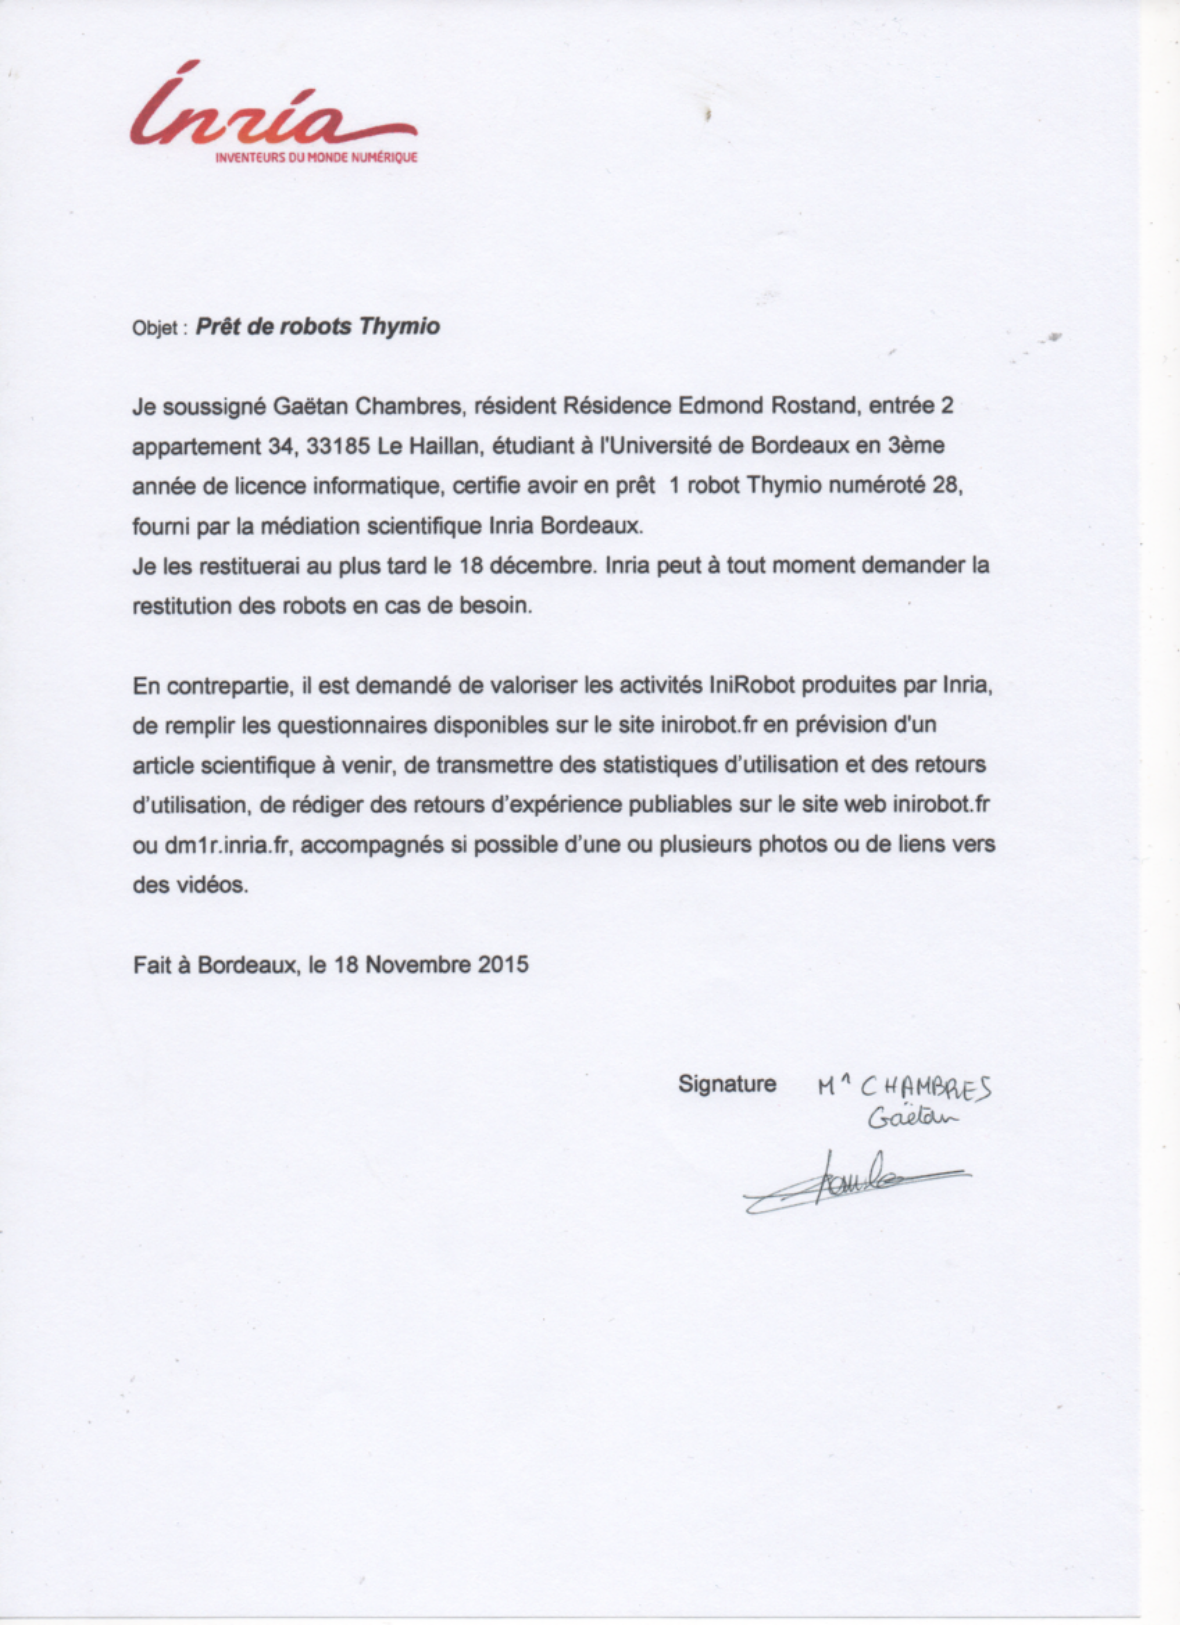
\includegraphics[width=0.9\textwidth]{pret.png}

\end{document}
